\documentclass[answers]{exam}
\usepackage[utf8]{inputenc}
\usepackage[english]{babel}
\usepackage{amsmath}
\usepackage{mathtools, amsthm}
\usepackage{amsfonts}
\usepackage{amssymb}
\usepackage{mathrsfs}
\usepackage{tcolorbox}


\newtheorem{theorem}{Theorem}[section]
\newtheorem{corollary}{Corollary}[theorem]
\newtheorem{lemma}[theorem]{Lemma}
\renewcommand{\qedsymbol}{$\blacksquare$}
\begin{document}
    %% \union - Example: \union{j \in J}{A_j}
\newcommand{\union}[2]{\underset{#1}\bigcup #2}

%% \inter - like \union, but with \bigcap
\newcommand{\inter}[2]{\underset{#1}\bigcap #2}
    \begin{questions}

        \question{
            The given diagram consists of a square of length
            10 cm and arcs of four circle of radius 10 cm.
            Find the area of the largest circle which can be fit
            into the shaded region.
            \begin{wrapfigure}{r}{5.5cm}
                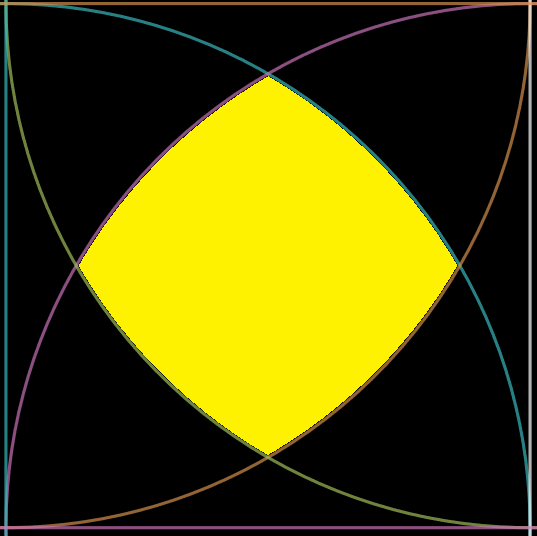
\includegraphics[scale=0.5]{questionmath.PNG}
                \end{wrapfigure}
        }
        

        \begin{solution}
                Since the diagonal of the square is $10\sqrt{2}$ and
            the radius of each circle is 10, we find that the length
            $2r=10\sqrt{2}-2y= 10\sqrt{2}-2(10\sqrt{2}-10) \implies
            r=10-5\sqrt{2}$ is symmetrical,
            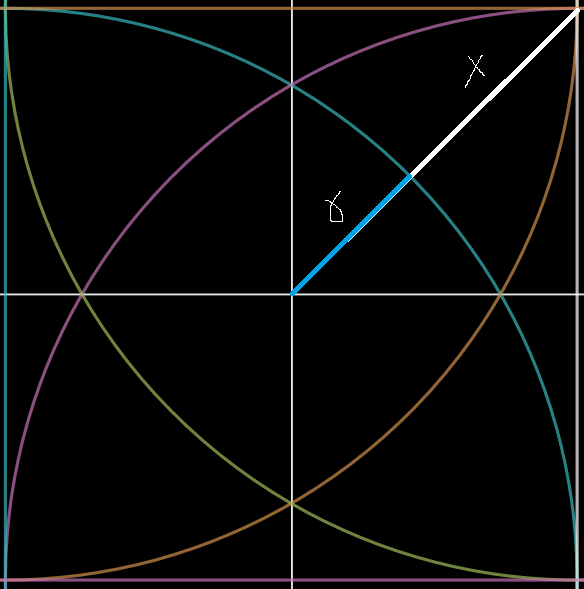
\includegraphics[width=2in]{questionmath125.png}

            \begin{minipage}{.69\textwidth}
                However, since it's not obvious that the circle we
                have found above is inside the shaded region, we will
                use Lagrange's multipliers method to minimize the distance
                from the center of the square to one of the arcs. This
                will show that the circle is inscribed inside the shaded
                region.
                Here, assume that the center of the square coincides
                with the origin in $\mathbb{R}^2$.
                We'll only consider the first quadrant and hence the arc
                that surrounds the shaded region in this quadrant
                will be an arc of the circle
                $(x+5)^2+(y+5)^2 =10^2$
                Now, we only need to minimize the function
                $d(x,y)=x^2+y^2$ with the above parameter.

                Using Lagrange's multipliers, we have
                $$\nabla\cdot d = \lambda\nabla\cdot g$$
                where $g(x,y)=(x+5)^2+(y+5)^2 -10^2$.
                This gives
                $$(2x,2y)=\lambda(2x+10,2y+10)$$
                So, $x=y=5\lambda/(1-\lambda)$. Substituting these for
                $g$ gives
                \begin{align*}
                    &2\left(\frac{5\lambda}{1-\lambda}+5\right)^2=100\\
                    \text{or}\quad&2\lambda^2-4\lambda+1=0
                    \implies \lambda = 
                \end{align*}
            \end{minipage}
            \begin{minipage}{.3\textwidth}
                \begin{flushright}
                    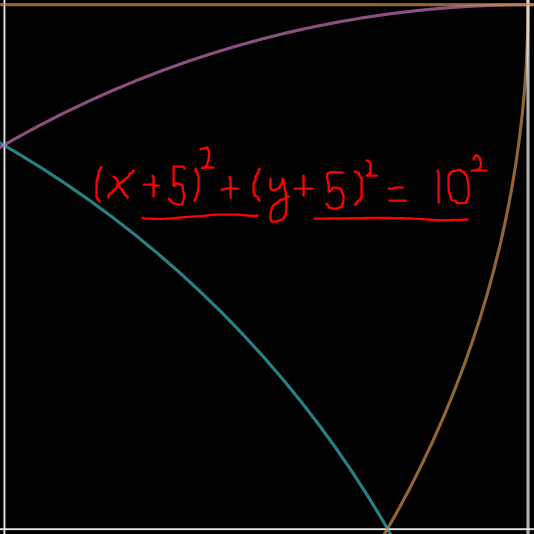
\includegraphics[width=1.5in]{questionmath3.PNG}
                \end{flushright}
            \end{minipage}
            

            
        \end{solution}
    \end{questions}
\end{document}